\documentclass[a0, portrait]{a0poster}
%%%Load packages
\usepackage{multicol} 			%3-column layout
\usepackage[left=1.5cm,right=1.5cm,bottom=0cm,top=0cm]{geometry}			%Reset margins
%\usepackage{fontspec} % For loading fonts
%\setmainfont[SmallCapsFont = Fontin SmallCaps, Ligatures=TeX]{Fontin} % Main document font
\usepackage[scaled=1]{helvet}
\usepackage[x11names]{xcolor}				%Needed for colour boxes & coloured text
\usepackage{graphicx}%%%Define colours and lengths
\usepackage[export]{adjustbox}
\usepackage{authblk}
    \usepackage{amsmath} % Equations
    \usepackage{amssymb} % Equations
\usepackage{bbm} %mathbbm
\usepackage{anyfontsize}
\usepackage{array, booktabs}
\usepackage[utf8]{inputenc}
\usepackage[russian]{babel}
\usepackage{tcolorbox}
\usepackage{mathtools}
\usepackage[hidelinks, linktoc=all, russian]{hyperref}
\usepackage{cleveref}
\usepackage{capt-of}
\usepackage[font=small,labelfont=bf]{caption}
\usepackage{subcaption}
\captionsetup[subfigure]{labelformat=parens}

\definecolor{headingcol}{rgb}{0.4, 0.57, 0.83}			%Colour of main title
\definecolor{titlecol2}{HTML}{CC181E}			%Colour of main title

\definecolor{titlecol}{rgb}{0.3, 0.47, 0.73}			%Colour of main title
\definecolor{boxcol}{rgb}{0.7,0.2,0.2}		%Edge-colour of box and top banner
\fboxsep=1cm							%Padding between box and text
\setlength{\columnsep}{2cm}				%Set spacing between columns
\renewcommand{\familydefault}{\sfdefault}	%Set main text to sans-serif


\newenvironment{frshaded}{%
\def\FrameCommand{\fboxrule=\FrameRule\fboxsep=\FrameSep \fcolorbox{framecolor}{shadecolor}}%
\MakeFramed {\FrameRestore}}%
{\endMakeFramed}

\renewcommand{\figureautorefname}{Fig.}%
\renewcommand{\figurename}{Fig.}

\graphicspath{{Pictures/}}

\newcommand{\diff}{\,\mathrm{d}} 	
 \renewcommand{\figureautorefname}{Fig.}%
\renewcommand*\thesection{\arabic{section}}
\DeclarePairedDelimiter\bra{\langle}{\rvert}
\DeclarePairedDelimiter\ket{\lvert}{\rangle}
\DeclarePairedDelimiterX\braket[2]{\langle}{\rangle}{#1 \delimsize\vert #2}
\newcommand{\rbrkt}[1]{\left( #1 \right)}
\newcommand{\sbrkt}[1]{\left[ #1 \right]}

\begin{document}

\begin{center}
\vspace*{-2cm}
\hspace*{-2cm}\includegraphics[width=1.2\textwidth]{Black_Landscape}
\end{center}


%%% Title
\begin{minipage}{0.65\textwidth}					
\vspace{-11cm}
\begin{tabular}[t]{l}
{\color{headingcol}\fontsize{68}{70}\selectfont Аналоговое моделирование цепочки Изинга при помощи трансмонов}\\
\\
{\hspace{1cm} \color{white}\large Г. Федоров\textsuperscript{1,2}, Е. Егорова\textsuperscript{1,2}, А. Доброносова\textsuperscript{4}, Н. Орликовский\textsuperscript{4}, А. Устинов\textsuperscript{1}} \\
\\
{\hspace{1.2cm}\color{white}\large \hspace{0.5cm} \textsuperscript{1}\textit{Российский квантовый центр} \hspace{0.5cm} \textsuperscript{2}\textit{Московский физико-технический институт} \hspace{0.5cm} 
\textsuperscript{3}\textit{Московский Государственный Технический Университет имени Н. Э. Баумана}}
\end{tabular}
\end{minipage}
%%% Logos
\hspace{19cm}
\begin{minipage}{0.2\textwidth}
\vspace{-11cm}
\begin{tabular}{c c}
\includegraphics[height=0.05\textheight]{logo}
\end{tabular}
\end{minipage}


\vspace{-1.5cm}
\begin{multicols}{2}	

%%%Column1

%%%%%%%%%%%%%%%%%% Introduction

\tcbset{colframe=titlecol, colback=white}
\begin{tcolorbox}[left=1cm, right=1cm, top=0.5cm, bottom=0.5cm, 
                  title={\Large Предисловие}, bottomtitle=.5cm,toptitle=.5cm]
\begingroup
\setlength{\columnsep}{1cm}
В настоящее время применение сверхпроводящих кубитов, как правило, ограничивается тестированием основных принципов квантовых вычислений, демонстрацией их в качестве концептуальных проектов и разработкой масштабируемых программных и аппаратных интерфейсов. Однако существует и альтернативное решение, включающее использование неотъемлемых квантовых свойств таких устройств для экспериментального изучения фундаментальных физических моделей. В последние годы были продемонстрированы первые успешные попытки\cite{li2018perfect}\cite{macha2014implementation}\cite{roushan2017spectroscopic} использования небольших массивов сверхпроводящих кубитов для наблюдения квантового аналогового поведения. В данной работе исследуется чип для экспериментального моделирования кристаллической структуры, многочастичной локализации (MBL) и свойств переноса тепла в цепочке трансмонов с ХХ связью. Первые результаты затронут спектроскопические свойства системы.
\endgroup
\end{tcolorbox}

%%%%%%%%%%%%%%%%%% Idea

\tcbset{colframe=titlecol}
\begin{tcolorbox}[left=1cm, right=1cm, top=0.5cm, bottom=0.5cm, 
                  title={\Large Контекст исследования}, bottomtitle=.3cm,toptitle=.5cm
                  ]
\begin{tabular}{cc}
	\begin{minipage}{0.5\textwidth}
		Гамильтониан пяти трансмонов, взаимодействующих только с ближайшими соседями, можно записать в виде суммы гамильтониана трансмонов без и с взаимодействием:               
		
		$$\hat{H}_{full} = \hat{H}_{single} + \hat{H}_{interaction},
		$$ где $
		\hat{H}_{single} = \sum_{i=1}^5 \hat{1}_1 \otimes \hat{1}_2 \otimes...\otimes \hat{H}_{i_0} \otimes...\otimes \hat{1}_5,
		$ $$
		\hat{H}_{int} = \sum_{i=1}^{4} \frac{e^2 M^{-1}_{i,j=i+1}}{2} \hat{1}_1 \otimes \hat{1}_2 \otimes...\otimes \hat{n}_{i} \otimes \hat{n}_{j} \otimes...\otimes \hat{1}_5.
		$$Здесь $\hat{H}_{i_0}$ - гамильтониан одного трансмона а $M^{-1}_{i,j=i+1}$ - элемент обратной матрицы емкости.
		Гамильтониан Изинга можно записать как $$
		H = -\frac{1}{2}\sum_{i}h_i\sigma_{z,i}+\hbar\sum_{i}J_{x,i}\sigma_{x,i}\sigma_{x,i+1},
		$$ где $
		J_{y,i},J_{z,i}=0
		$. Так как два вышеописанных гамильтониана имеют схожую структуру, то становится возможным осуществлять аналоговое моделирование спиновой цепочки.
	\end{minipage}
	&
	\begin{minipage}{0.5\textwidth}
		\centering
		\includegraphics[width=\textwidth]{chain_without_anticross}
		\begingroup
		\captionsetup[figure]{width=\textwidth}
		
		\captionof{figure}{Спектр пятикубитной цепочки. Первые 20 уровней.}
		\endgroup
	\end{minipage}
\end{tabular}
\end{tcolorbox}


%%%%%%%%%%%%%%%%%% Sample design
\tcbset{colframe=titlecol}
\begin{tcolorbox}[left=1cm, right=1cm, top=0.5cm, bottom=0.5cm, 
                  title={\Large Дизайн образца}, bottomtitle=.3cm,toptitle=.5cm
                  ]
Образец был изготовлен на кремниевой подложке с помощью электронной литографии и метода теневого напыления в чистой зоне МГТУ им. Баумана.

\vspace{1cm}
\begin{minipage}{\textwidth}
\centering
\includegraphics[width=\textwidth]{design}
\begingroup
\captionsetup[figure]{width=\textwidth}

\captionof{figure}{\textbf{(a)} Дизайн образца: 5 трансмонов, выстроенных в цепочку с поперечной связью и возможностью считывания состояния каждого кубита. \textbf{(б)} \textbf{(в)} Увеличенные области со СКВИДом и потоковой линией смещения. \textbf{(г)} Образец, соединенный с держателем с помощью ультразвуковой сварки.}
\endgroup
\end{minipage}

\end{tcolorbox}



%%%%%%%%%%%%%%%%%% Моделирование в Максвелле
\tcbset{colframe=titlecol}
\begin{tcolorbox}[left=1cm, right=1cm, top=0.5cm, bottom=0.5cm, 
	title={\Large Расчет емкостей в ANSYS Maxwell}, bottomtitle=.3cm,toptitle=.5cm
	]
	Матрица емкости пяти кубитов может быть записана следующим образом:
	\[ 
	M =  \rbrkt{\begin{matrix}
		\sum_{k=1}^5 C_{q_{1k}}&-C_{q_{12}}&C_{q_{13}}&C_{q_{14}}&C_{q_{15}}\\
		-C_{q_{12}}&\sum_{k=1}^5 C_{q_{2k}}&-C_{q_{23}}&-C_{q_{24}}&C_{q_{25}}\\
		-C_{q_{13}}&-C_{q_{23}}&\sum_{k=1}^5 C_{q_{3k}}&-C_{q_{34}}&C_{q_{35}}\\
		-C_{q_{14}}&-C_{q_{24}}&-C_{q_{34}}&\sum_{k=1}^5 C_{q_{4k}}&-C_{q_{45}}\\
		-C_{q_{15}}&-C_{q_{25}}&-C_{q_{35}}&-C_{q_{45}}&\sum_{k=1}^5 C_{q_{5k}}
		\end{matrix} }.
	\]
	Для контроля взаимодействия преимущественно с ближайшими соседями был проведен расчет емкостей имеющегося дизайна.

	
	\vspace{1cm}
	\begin{minipage}{\textwidth}
		\centering
		\includegraphics[width=\textwidth]{maxw1}
		\begingroup
		\captionsetup[figure]{width=\textwidth}
		
		\captionof{figure}{Расчет емкостей методом конечных элементов. Таблице с матрицей емкости в фФ.}
		\endgroup
	\end{minipage}


		\centering
		\vspace{1cm}

		\begin{tabular}{|c|c|c|c|c|c|c|}
			\hline
			№/№ & $C_{q1}$ & $C_{q2}$ & $C_{q3}$ & $C_{q4}$ & $C_{q5}$ & $C_{ground}$ \\
			\hline
			$C_{q1}$ & 204.32 & -1.6719 & -0.01648 & -0.0023559 & -0.00041832 & -202.63  \\
			\hline
			$C_{q2}$ & -1.6719 & 184.42 & -1.5558 & -0.015993 & -0.0023771 & -181.18\\ 
			\hline
			$C_{q3}$  & -0.01648 & -1.5558 & 208.25 & -1.4411 & -0.016563 & -205.22\\
			\hline
			$C_{q4}$  & -0.0023559 & -0.015993 & -1.4411 & 196.76 & -1.1688 & -194.13\\
			\hline
			$C_{q5}$  & -0.00041832 & -0.0023771 & -0.016563 & -1.1688 & 209.54 & -208.36\\
			\hline
			$C_{ground}$  & -202.63 & -181.18 & -205.22 & -194.13 & -208.36 & 991.51\\
			\hline
		\end{tabular}

	

	
\end{tcolorbox}




%%%%%%% Схема
\tcbset{colframe=titlecol}
\begin{tcolorbox}[left=1cm, right=1cm, top=0.5cm, bottom=0.5cm, 
	title={\Large Схема установки}, bottomtitle=.3cm,toptitle=.5cm
	]
	
	
	\vspace{1cm}
	\begin{minipage}{\textwidth}
		\centering
		\includegraphics[width=\textwidth]{exp_scheme}
		\begingroup
		\captionsetup[figure]{width=\textwidth}
		
		\captionof{figure}{Слева изображена собранная схема для спектроскопических и импульсных измерений, в правой- аттенюация и фильтрация линий на ступенях криостата и непосредственно образец в держателе с катушкой.}
		\endgroup
	\end{minipage}
	
\end{tcolorbox}


%%%%%%%Измерения
\tcbset{colframe=titlecol}
\begin{tcolorbox}[left=1cm, right=1cm, top=0.5cm, bottom=0.5cm, 
	title={\Large Эксперимент}, bottomtitle=.3cm,toptitle=.5cm
	]
	
	\vspace{1cm}
	\begin{minipage}{\textwidth}
		\centering
		\includegraphics[width=\textwidth]{crosstalks}
		\begingroup
		\captionsetup[figure]{width=\textwidth}
		
		\captionof{figure}{Зависимость картин однотоновой спектроскопии кубитов от используемой потоковой линии смещения.}
		\endgroup
	\end{minipage}
	
\end{tcolorbox}

%%%%%%%% Conclusion

\tcbset{colframe=titlecol}
\begin{tcolorbox}[left=1cm, right=1cm, top=0.5cm, bottom=0.5cm, 
                  title={\Large Выводы}, bottomtitle=.5cm,toptitle=.5cm
                  ]

???

\end{tcolorbox}

\tcbset{colframe=titlecol}
\begin{tcolorbox}[left=1cm, right=1cm, top=0.5cm, bottom=0.5cm, 
                  title={\Large Литература}, bottomtitle=.5cm,toptitle=.5cm
                  ]
\bibliographystyle{Science}
\bibliography{poster2019.bib}
\end{tcolorbox}

\end{multicols}


\end{document}